\documentclass[10pt, uplatex, dvipdfmx]{jsarticle}
\usepackage{../mypackage}

\graphicspath{{../pictures}}

\setcounter{section}{2}

\begin{document}


\section{分数関数の積分}

$\ds \frac{\text{多項式}}{\text{多項式}}$ という形をした関数
は\textbf{分数関数}とか\textbf{有理関数}と呼ばれる.その積分の計算方法をまとめる.
% \[
%   \int \frac{dx}{(x-\alpha)^n}, \qquad \int \frac{Bx+C}{(x^2+bx+c)^n}\ dx
%   \qquad (n \text{ は自然数 })
% \]

\subsection{多項式の割り算}\label{subsec:division}

\begin{wrapfigure}{r}[0pt]{0.5\textwidth}
  \centering
  \includegraphics[width=7cm]{03/remainder.pdf}
\end{wrapfigure}
例えば,次のような分数関数 $f(x)$ を積分したい.
\[
  f(x) = \frac{x^5+3x^3-2x+1}{x^2+3x+2}
\]
この分子と分母の多項式としての次数を比べると
\[
  \text{ 分子の次数 }  \geqq \text{ 分母の次数} 
\]
である.このような場合は,まず右のように分子を分母で割った商と余
りを計算しておく.この計算により $f(x)$ の分子が
\[
  x^5+3x^3-2x+1 = (x^3-3x^2+10x-24)(x^2+3x+2) + 50x+49
\]
と書けるので
\[
  f(x) = \frac{ (x^3-3x^2+10x-24)(x^2+3x+2) + 50x+49}{x^2+3x+2} = x^3-3x^2+10x-24 + \frac{50x+49}{x^2+3x+2}
\]
と変形できる.よって,$f(x)$ の積分は
\[
  \int f(x) \ dx = \frac{1}{4}x^4 - x^3-5x^2-24x + \int
  \frac{50x+49}{x^2+3x+2} \ dx
\]
となり,もともとの $\ds \frac{\text{ $5$ 次式}}{\text{ $2$ 次式}}$ の積
分が $\ds \frac{\text{$1$ 次式}}{\text{$2$ 次式}}$ の積分に帰着されている.より一般に,分数関数が
\[
  f(x) = \frac{g(x)}{h(x)}
\]
と,$2$ 個の多項式 $g(x)$ と $h(x)$ の比で書けるとき,多項式の割り算を実行して
\[
  g(x) = q(x) h(x) + r(x), \quad \deg r(x) < \deg h(x)
\]
を満たす多項式 $q(x)$ と $r(x)$ を計算することができる.$q(x)$ が商
で,$r(x)$ が余りである.ただし,初めから $\deg g(x) < \deg h(x)$ であ
れば,$q(x)=0, \; r(x) = h(x)$ である.これらによって
\[
  f(x) = \frac{q(x)h(x)+r(x)}{h(x)} = q(x) + \frac{r(x)}{h(x)}
\]
と,$f(x)$ を「多項式」と「分子の次数 $<$ 分母の次数となる分数関数」の和に分けることができる.つまり,
\[
  \text{ 分子の次数 } < \text{ 分母の次数}
\]
となる分数関数の積分が計算できれば,原理的にはどんな分数関数の積分も計算できる.

\subsection{部分分数分解}\label{subsec:partfrac}

分数関数 $\ds f(x) = \frac{x^5+3x^2-2x+1}{x^2+3x+2}$ の積分を完成させよう.先ほど見たように
\[
  \int f(x) \ dx = \frac{1}{4}x^4-x^3-5x^2-24x + \int \frac{50x+49}{x^2+3x+2} \ dx
\]
なので,最後に残った積分
\[
  \int \frac{50x+49}{x^2+3x+2}\ dx
\]
を計算してしまえばよい.まず,分母が
\[
  \frac{50x+49}{x^2+3x+2} = \frac{50x+49}{(x+1)(x+2)}
\]
と因数分解できる.これをさらに
\[
  \frac{50x+49}{(x+1)(x+2)} = \frac{A}{x+1} + \frac{B}{x+2}
\]
という簡素な分数関数の和に分けることができる.特に,左辺が
\[
  \text{ 分子の次数 } < \text{ 分母の次数}
\]
なので,右辺に並ぶ分数関数も全てそうなる.従って,$A, B$ は共に $0$ 次,つまり定数である.実際,
上式の右辺を通分すれば
\[
  \frac{A}{x+1} + \frac{B}{x+2} = \frac{A(x+2)+B(x+1)}{(x+1)(x+2)} = \frac{(A+B)x + (2A+B)}{(x+1)(x+2)}
\]
となるので,分子の係数を比較して以下の連立1次方程式を解けばよい.
\[
  \begin{cases}
    A+B=50\\
    2A+B=49
  \end{cases} \quad \left( \Longleftrightarrow \left[
      \begin{array}{rr}
        1 & 1\\
        2 & 1
      \end{array}
      \right] \left[
        \begin{array}{r}
          A\\
          B
        \end{array}
      \right] = \left[
        \begin{array}{r}
          50\\
          49
        \end{array}
      \right] \right)
\]
これは簡単に解けて,$A=-1, \; B=51$ である. つまり,
\[
  \frac{50x+49}{(x+1)(x+2)} = -\frac{1}{x+1} + \frac{51}{x+2}
\]
なのでその積分は
\[
  \int \frac{50x+49}{(x+1)(x+2)} \ dx = -\int\frac{dx}{x+1} + 51\int
  \frac{dx}{x+2}= -\log|x+1| +51\log|x+2|
\]
と計算できる.これによって,$f(x)$ の積分が以下の通り完成する.
\[
  \int \frac{x^5+3x^2-2x+1}{x^2+3x+2} \ dx = \frac{1}{4}x^4 -
  x^3-5x^2-24x -\log|x+1| + 51 \log |x+2|
\]

\newpage

別の例として,次の分数関数 $g(x)$ を積分してみよう.
\[
  g(x) = \frac{6x^2+x+1}{x^3+x^2+x+1}
\]
これは初めから
\[
  \text{ 分子の次数 } < \text{ 分母の次数}
\]
なので,多項式の割り算を実行する必要はない.分母が
\[
  x^3+x^2+x+1 = x^2(x+1) + x+1 = (x^2+1)(x+1)
\]
と因数分解できるので,$g(x)$ を次の形に分解する.
\[
  \frac{6x^2+x+1}{(x+1)(x^2+1)} = \frac{\bigcirc}{x+1} + \frac{\square}{x^2+1}
\]
右辺はどちらも「分子の次数 $<$ 分母の次数」としたいの
で,$\bigcirc$ は定数($0$ 次)で,$\square$ は $1$ 次以下の多項式である.そ
こで,$\bigcirc = A, \; \square = Bx+C$ とおく.つまり,以下を満たす定数 $A,B,C$ を見つければよい.
\[
  \frac{6x^2+x+1}{(x+1)(x^2+1)} = \frac{A}{x+1} + \frac{Bx+C}{x^2+1}
\]
結果的にもしも $B=0$ となれば $\square$ は定数だったことになるが,それは計算
してみないとわからないので,とりあえずは $\square$ を $1$ 次式としておく.上式の右辺を通分すれば
\[
  \frac{6x^2+x+1}{(x+1)(x^2+1)} = \frac{A(x^2+1) +
    (x+1)(Bx+C)}{(x+1)(x^2+1)} = \frac{(A+B)x^2 + (B+C)x +
    (A+C)}{(x+1)(x^2+1)}
\]
となるので,分子の係数を比較して以下の連立1次方程式を解けばよい.
\[
  \begin{cases}
    A+B=6\\
    B+C=1\\
    A+C=1
  \end{cases} \quad \left( \Longleftrightarrow \left[
      \begin{array}{rrr}
        1 & 1 & 0\\
        0 & 1 & 1\\
        1 & 0 & 1
      \end{array}
    \right]\left[
      \begin{array}{r}
        A\\
        B\\
        C
      \end{array}
    \right] = \left[
      \begin{array}{r}
        6\\
        1\\
        1
      \end{array}
    \right]
  \right)
\]
これは簡単に解けて,$A=3, \; B=3, \; C=-2$ である.つまり,
\[
  g(x) = \frac{6x^2+x+1}{(x+1)(x^2+1)} = \frac{3}{x+1} + \frac{3x-2}{x^2+1}
\]
なので,その積分は以下のように計算できる.
\[
  \begin{aligned}
    \int g(x) \ dx
    &= 3\int \frac{dx}{x+1} + 3\int \frac{x}{x^2+1} \ dx - 2 \int \frac{dx}{x^2+1}\\[1ex]
    &  =3\log|x+1| + \frac{3}{2}\int \frac{2x}{x^2+1}\ dx - 2 \tan^{-1}x\\[1ex]
    &= 3\log|x+1| + \frac{3}{2} \int \frac{(x^2+1)'}{x^2+1}\ dx - 2\tan^{-1}x\\[1ex]
    &  =3 \log|x+1| + \frac{3}{2} \log(x^2+1) -2\tan^{-1}x 
  \end{aligned}
\]

\newpage

より一般に,分数関数 $\ds \frac{Q(x)}{P(x)}$の分母が互いに素な $r$ 個の多項式の積として
\[
  P(x) = P_1(x)P_2(x) \cdots P_r(x)
\]
と因数分解されれば,分数関数を多項式 $Q_0(x)$ といくつかの分数関数の和として
\[
  \frac{Q(x)}{P(x)} = Q_0(x) + \frac{Q_1(x)}{P_1(x)} + \frac{Q_2(x)}{P_2(x)} +
  \cdots + \frac{Q_r(x)}{P_r(x)} \quad (\deg Q_i(x) < \deg P_i(x), \; i=1,2, \ldots, r)
\]
となるように分解できる.これを分数関数 $\ds
\frac{Q(x)}{P(x)}$ の\textbf{部分分数分解}という.特に,$P(x), Q(x)$ が
実数係数の多項式なら,各 $P_i(x), Q_i(x)$ も実数係数の多項式で,各分
母 $P_i(x)$ が次のいずれかの形になるまで分解できる.
\[
   (x-\alpha)^n \quad \text{ または } \quad (x^2+bx+c)^n \qquad (n \text{ は自然数 })
\]
従って,部分分数分解の多項式以外の各項は以下のいずれかの形をしている.
\[
  \frac{ \bigcirc x^{n-1} + \square x^{n-2} + \cdots + \triangle}{(x-\alpha)^n} \quad \text{ または } \quad
  \frac{\bigcirc x^{2n-1} + \square x^{2n-2} + \cdots + \triangle}{(x^2+bx+c)^n}
\]
さらに,例えば
\[
  \begin{aligned}
    \frac{x^2}{(x-1)^3}
    &= \frac{(x+1)(x-1)+1}{(x-1)^3} = \frac{x+1}{(x-1)^2} + \frac{1}{(x-1)^3}
      = \frac{(x-1)+2}{(x-1)^2} + \frac{1}{(x-1)^3} \\[1ex]
    &= \frac{1}{x-1} + \frac{2}{(x-1)^2} + \frac{1}{(x-1)^3}\\[5ex]
    \frac{x^3+2x+1}{(x^2+x+1)^2}
    &= \frac{(x-1)(x^2+x+1)+2x+2}{(x^2+x+1)^2} = \frac{x-1}{x^2+x+1} + \frac{2x+2}{(x^2+x+1)^2}
  \end{aligned}
\]
のように分解できるので,任意の分数関数は各項が多項式か以下のいずれかの形になるまで分解できる.
\begin{equation}\label{eq:basic-forms}
  \frac{\bigcirc}{(x-\alpha)^n} \quad \text{ または } \quad
  \frac{\square x + \bigtriangleup}{(x^2+bx+c)^n} \qquad (n \text{ は自然数 })
\end{equation}
よって,これらの形の分数関数の積分が計算できるようになっておけば,どん
な分数関数も積分できる(と言い切りたいが,実際には「どんな分数関数も」
は言い過ぎで,分母の次数が高いとその因数分解が難しい).

\newpage

\subsection{基本形の積分}\label{subsec:basic}

分数関数の積分は以下の基本形の積分に帰着できるので,これらの計算方法を確立していく.
\[
  [1] \int\frac{dx}{(x-\alpha)^n} \qquad \qquad [2] \int \frac{Bx+C}{(x^2+bx+c)^n}\ dx \qquad
  ( \text{ いずれも $n$ は自然数 } )
\]

\vspace{1zh}

まず,[1]については,例えば以下のように簡単に計算できる.
\[
  \int \frac{dx}{x-1} = \log|x-1|, \qquad \int \frac{dx}{(x-1)^2} = -(x-1)^{-1}, \qquad
  \int \frac{dx}{(x-1)^3} = -\frac{1}{2} (x-1)^{-2}
\]

\vspace{1zh}

次に,[2]ではまず分母の括弧の中の2次式を以下のように平方完成する.
\begin{equation}\label{eq:sq-comp}
  x^2+bx+c = (x-\alpha)^2 + \beta
\end{equation}
ここで,$\beta \leqq 0$ となる場合は右辺が因数分解できるので[1]の場合
に帰着される.そこで,$\beta >0$ かつ $n=1$ の場合の例として次の積分を計算する.
\[
  \int \frac{dx}{x^2+x+1}
\]
この場合,分母の2次式は
\[
  x^2+x+1 = \left( x+ \frac{1}{2}\right)^2 + \frac{3}{4}
\]
と平方完成できるので,$\ds u=x+\frac{1}{2}$ とおいて置換積分を適用すれ
ば,積分は次のように計算できる.
\[
  \int \frac{dx}{x^2+x+1} = \int \frac{du}{u^2+ \frac{3}{4}} = \frac{2}{\sqrt{3}} \tan^{-1} \frac{2u}{\sqrt{3}}
  = \frac{2}{\sqrt{3}} \tan^{-1} \frac{2x+1}{\sqrt{3}}
\]
ここで,次の積分公式を $a= \sqrt{3}/2$ として使った
(\ref{subsec:fundamental}節後半で導出した公式の一般化).
\[
  \int \frac{dx}{x^2+a^2} = \frac{1}{a} \tan^{-1} \frac{x}{a} \quad (a >0)
\]

\vspace{1zh}

さらに,この結果を利用して [2] としてもう少し一般的な形の次の積分を計算する.
\[
  \int \frac{x+1}{x^2+x+1} \ dx
\]
分母の2次式 $x^2+x+1$ を微分すると1次式 $2x+1$ になることを活用して
\[
  \int \frac{ x+1}{x^2+x+1} \ dx  = \int \frac{\frac{1}{2}\left( 2x+1\right) + \frac{1}{2}}{x^2+x+1} \ dx
  = \frac{1}{2} \int \frac{(x^2+x+1)'}{x^2+x+1}\ dx + \frac{1}{2}\int\frac{dx}{x^2+x+1}
\]
と変形できる.最右辺の第1項は $\ds \frac{f'(x)}{f(x)} = \left( \log \left|f(x)\right|
\right)'$ の形であり,第2項は直前に計算したばかりなので,
\[
  \int \frac{x+1}{x^2+x+1}\ dx = \frac{1}{2}\log\left| x^2+x+1\right|
  + \frac{1}{\sqrt{3}}\tan^{-1}\frac{2x+1}{\sqrt{3}}
\]
と計算できる.ちなみに,$x^2+x+1>0$ なので,$\left| x^2+x+1 \right|= x^2+x+1 $ である.

\newpage

残りの場合を片付けてしまおう.つまり,[2]としてより一般的な以下の形の積分を計算したい.
\begin{equation}\label{eq:general-quadratic}
  \int \frac{Bx+C}{(x^2+bx+c)^n} \qquad (n \geqq 2)
\end{equation}
例として,次の積分を計算していく.
\[
  \int \frac{x+2}{(x^2+x+1)^2} \ dx
\]
まず,先程と同様に,分母に現れる2次式 $x^2+x+1$ を微分すると1次式 $2x+1$ になることを活用して
\[
  \int \frac{x+2} {(x^2+x+1)^2} \ dx = \int \frac{ \frac{1}{2} (2x+1) + \frac{3}{2}}{(x^2+x+1)^2} \ dx
  = \frac{1}{2} \int \frac{ (x^2+x+1)'}{(x^2+x+1)^2} \ dx + \frac{3}{2} \int \frac{dx}{(x^2+x+1)^2}
\]
と変形できる.この最右辺の第1項の被積分関数は $\ds  \frac{f'(x)}{f(x)^2} = \left( -\frac{1}{f(x)}\right)'$ という形なので
\[
  \int \frac{x+2}{(x^2+x+1)^2} \ dx = \frac{-\frac{1}{2}}{x^2+x+1} + \frac{3}{2}\int\frac{dx}{(x^2+x+1)^2}
\]
と計算できる.最後に残った積分は,先程と同様に,$\ds u=x+\frac{1}{2}$ とおけば置換積分によって
\[
  \int \frac{dx}{(x^2+x+1)^2} = \int \frac{du}{\left(u^2+\frac{3}{4}\right)^2}
\]
と変換できる.ここで突然だが,この積分を計算するために次のような部分積分の計算を行う.
\begin{equation}\label{eq:lin2sq}
  \begin{aligned}
    \int \frac{du}{u^2+\frac{3}{4}}
    &= \int (u)'
      \frac{1}{u^2+\frac{3}{4}} \ dx = \frac{u}{u^2+\frac{3}{4}} - \int u
      \left(\frac{1}{u^2+\frac{3}{4}}\right)' \ du
      = \frac{u}{u^2+\frac{3}{4}} +\int \frac{2u^2}{\left(u^2+\frac{3}{4}\right)^2} \ du\\
    &= \frac{u}{u^2+\frac{3}{4}} + 2\int \frac{u^2 + \frac{3}{4} - \frac{3}{4}}{\left(u^2+\frac{3}{4}\right)^2} \ du
      = \frac{u}{u^2+\frac{3}{4}} + 2\left( \int \frac{du}{u^2+\frac{3}{4}}
      - \frac{3}{4}\uwave{\int \frac{du}{\left(u^2+\frac{3}{4}\right)^2}} \right)
  \end{aligned}
\end{equation}
波線部に計算したかった積分が現れた.上式の最左辺と最右辺が等しいので,波線部について解いて
\[
  \int  \frac{du}{\left( u^2 + \frac{3}{4}\right)^2} = \frac{2}{3} \left( \frac{u}{u^2+\frac{3}{4}} + \int \frac{du}{u^2+\frac{3}{4}}\right)
\]
を得る.右辺の最後に現れた積分は先ほど計算したので
\[
  \int \frac{du}{\left( u^2+\frac{3}{4}\right)^2} = \frac{2}{3}\left(
    \frac{u}{u^2+\frac{3}{4}} +
    \frac{2}{\sqrt{3}}\tan^{-1}\frac{2}{\sqrt{3}}u\right) 
\]
である.以上から,最終的に以下が得られる.
\[
  \begin{aligned}
    \int \frac{x+2}{(x^2+x+1)^2} \ dx
    & = \frac{-\frac{1}{2}}{x^2+x+1} + \frac{3}{2}\int \frac{du}{\left(u^2+\frac{3}{4}\right)^2}\\[2ex]
    &  = \frac{-\frac{1}{2}}{x^2+x+1} + \frac{u}{u^2+\frac{3}{4}} + \frac{2}{\sqrt{3}} \tan^{-1}\frac{2}{\sqrt{3}}u\\[2ex]
    & = \frac{-\frac{1}{2}}{x^2+x+1} + \frac{x+\frac{1}{2}}{x^2+x+1} + \frac{2}{\sqrt{3}}\tan^{-1} \frac{2x+1}{\sqrt{3}}\\[2ex]
    & = \frac{x}{x^2+x+1} + \frac{2}{\sqrt{3}}\tan^{-1} \frac{2x+1}{\sqrt{3}}x
  \end{aligned}
\]

\newpage

より一般に,(\ref{eq:general-quadratic}) の形の積分は前ページの例と同様に小手先のテクニックを駆使して,最終的には
\[
  \int \frac{du}{(u^2+a^2)^n} \quad ( a>0 )
\]
という形の積分に帰着される.これを計算してもよいが,もう少しだけ式を簡単にしておこう.
\[
  \frac{1}{(u^2+a^2)^n} = \frac{1}{a^{2n}\left( \left(\frac{u}{a}\right)^2+1\right)^n}
\]
なので,$\ds t=\frac{u}{a}$ とおいて置換積分を適用すればこの積分は
\[
  \int \frac{du}{(u^2+a^2)^n} = \frac{1}{a^{2n}} \int \frac{a}{(t^2+1)^n} \ dt = \frac{1}{a^{2n-1}} \int \frac{dt}{(t^2+1)^n}
\]
と変換できる.つまり,各 $n=1,2,3, \ldots$ に対して
\[
  I_n := \int \frac{dt}{(t^2+1)^n} 
\]
が計算できればよい.そのために,(\ref{eq:lin2sq}) と同様に $I_{n}$ を部分積分して $I_{n+1}$ を生み出す.
\[
  \begin{aligned}
    I_{n}
    & = \int \frac{(t)'}{(t^2+1)^n} \ dt = \frac{t}{(t^2+1)^n} - \int t\left( \frac{1}{\left(t^2+1\right)^n}\right)' \ dt
      = \frac{t}{(t^2+1)^n} + \int \frac{2nt^2}{(t^2+1)^{n+1}} \ dt\\[2ex]
    & = \frac{t}{(t^2+1)^n} + 2n \int \frac{t^2+1 - 1}{(t^2+1)^{n+1}} \ dt
      =\frac{t}{(t^2+1)^n} + 2n \left( \int \frac{dt}{(t^2+1)^n} - \int \frac{dt}{(t^2+1)^{n+1}} \ dt\right)\\[2ex]
    &= \frac{t}{(t^2+1)^n} + 2n\left( I_n -  I_{n+1}\right)
  \end{aligned}
\]
これの最左辺と最右辺を結ぶ等式から,以下の漸化式が得られる.
\[
  I_{n+1} = \frac{1}{2n}\left( \frac{t}{(t^2+1)^n} + (2n-1)I_n\right)
\]
これが全ての自然数 $n$ について成り立ち,さらに
\[
  I_1 = \int \frac{dt}{t^2+1} = \tan^{-1}t
\]
から,以下のように $I_2, I_3, I_4, \ldots$ を次々と計算していくことができる.
\[
  \begin{aligned}
    I_2 &= \frac{1}{2}\left(\frac{t}{t^2+1} + I_1 \right) = \frac{1}{2}~ \frac{t}{t^2+1} + \frac{1}{2}\tan^{-1}t \\[1ex]
    I_3 &= \frac{1}{4}\left(\frac{t}{(t^2+1)^2} + 3 I_2\right)=\frac{1}{4}~\frac{t}{(t^2+1)^2}
          + \frac{3}{8}~\frac{t}{t^2+1} + \frac{3}{8} \tan^{-1} t \\[1ex]
    I_4 &= \frac{1}{6} \left( \frac{t}{(t^2+1)^3} + 5 I_3\right) = \frac{1}{6}~\frac{t}{(t^2+1)^3}
          + \frac{5}{24}~\frac{t}{(t^2+1)^2} + \frac{5}{16}~\frac{t}{t^2+1} + \frac{5}{16}\tan^{-1}t 
  \end{aligned}
\]
あるいは,結果として上記のように各 $I_n$ は
\[
  I_n = a_{n-1} ~\frac{t}{(t^2+1)^{n-1}} + a_{n-2} ~\frac{t}{(t^2+1)^{n-2}} + \cdots + a_1~ \frac{t}{t^2+1} + a_0 \tan^{-1}t
\]
という形に書けるということだけを覚えておけば,これの右辺を微分してそれが $\ds
\frac{1}{(t^2+1)^n}$ に等しくなるように定数 $a_0, a_1, \ldots,
a_{n-1}$ を定めることもできる.つまり,$n$ 個の変数 $a_0, a_1, \ldots,
a_{n-1}$ に関する連立1次方程式を解くことでこれらの積分を計算することもできる.

\newpage

\subsection{練習問題}

答えは次のページ

\vspace{1zh}

\begin{enumerate}
  \setlength{\itemsep}{2zh}
  

\item 次の分数関数を「多項式」と「分子の次数 $<$ 分母の次数となる分数関数」の和に分けよう.

  \vspace{1zh}

  \begin{enumerate}[(1)]
    \setlength{\itemsep}{3zh}
    
  \item $\ds \frac{x^4+x+4}{x^3+x^2+x+1}$

  \item $\ds \frac{3x^4+x^3+13x^2+5}{(x+1)(x^2+2x+4)}$

  \item $\ds \frac{8x^5 + 82 x^4 + 287 x^3 + 259 x^2 -304 x -361}{x^3 (x^2+8x+19)^2}$
    
  \end{enumerate}

\item 前問 2. の分数関数を多項式と (\ref{eq:basic-forms}) の形の分数関数たちの和に分解しよう.
  
\item 前問1.と 前々問 2. を踏まえて,次の積分の値を求めよう.

  \vspace{1zh}
  
  \begin{enumerate}[(1)]
    \setlength{\itemsep}{2zh}
    
  \item $\ds \int_{0}^{1} \frac{x^4+x+4}{x^3+x^2+x+1} \ dx$
    
  \item $\ds \int_{0}^{2} \frac{3x^4+x^3+13x^2+5}{(x+1)(x^2+2x+4)} \ dx$
    
  \item $\ds \int_{-3}^{-1} \frac{8x^5 + 82 x^4 + 287 x^3 + 259 x^2 -304 x -361}{x^3 (x^2+8x+19)^2} \ dx$
    
  \end{enumerate}
  
\end{enumerate}

\vspace{2zh}


「積分基本問題集 壱」$(27) \sim (35)$ も参考にしてください.

\newpage

\begin{center}
  \textbf{解答}
\end{center}

\begin{enumerate}
  \setlength{\itemsep}{2zh}
\item
  \begin{enumerate}[(1)]
    \setlength{\itemsep}{2zh}
    
  \item $\ds x-1 + \frac{x+5}{x^3+x^2+x+1}$

  \item $\ds 3x-8 + \frac{19x^2+36x+37}{(x+1)(x^2+2x+4)}$

  \item $\ds  (\; 0 \; + \; ) \; \frac{8x^5 + 82 x^4 + 287 x^3 + 259 x^2 -304 x -361}{x^3 (x^2+8x+19)^2}$
  \end{enumerate}

\item
  \begin{enumerate}[(1)]
    \setlength{\itemsep}{2zh}
    
  \item $\ds x-1 + \frac{2}{x+1} + \frac{-2x+3}{x^2+1}$

  \item $\ds 3x-8 + \frac{\frac{20}{3}}{x+1} + \frac{\frac{37}{3} x + \frac{31}{3}}{x^2+2x+4}$

  \item $\ds ( \; 0 \; + \; ) \; \frac{1}{x} + \frac{-1}{x^3} + \frac{-x}{x^2+8x+19} + \frac{-1}{(x^2+8x+19)^2}$
  \end{enumerate}

\item
  \begin{enumerate}[(1)]

    \setlength{\itemsep}{2zh}
    
  \item $\ds \frac{3}{4}\pi - \frac{1}{2} + \log 2$
    
  \item $\ds \frac{77}{6}\log 3 -10 - \frac{\sqrt{3}}{9} \pi$
    
  \item $\ds \frac{4}{9} + \frac{23\sqrt{3}}{108} \pi - \frac{3}{2} \log 3$
  \end{enumerate}
\end{enumerate}

\newpage

\subsection{(おまけ)特殊な置換積分たち}

置換積分によって分数関数の積分に帰着できるものは少なくない.例えば,次の積分を考える.
\[
  \int \frac{\cos x}{\sin x - 3 \cos x} \ dx
\]
これを計算するために(非常に突然だが)変数変換 $\ds u=\tan\frac{x}{2}$ を考える.このとき,
\[
  \frac{du}{dx} = \frac{1}{2}\left( 1+ \tan^2\frac{x}{2}\right) = \frac{1}{2}(1+u^2)
\]
である.さらに,$\cos x, \; \sin x$ が $u$ の式としてそれぞれ次のように書ける.
\[
  \begin{aligned}
    \cos x &= 2\cos^2\frac{x}{2} - 1 = \frac{2}{1+\tan^2\frac{x}{2}} -1= \frac{2}{1+u^2}-1 =\frac{1-u^2}{1+u^2}\\[2ex]
    \sin x &= 2 \left( \sin\frac{x}{2}\right) \left(\cos\frac{x}{2}\right)
             = 2~ \frac{\sin \frac{x}{2}}{\cos \frac{x}{2}}~ \cos^2 \frac{x}{2}
             = 2 \left(\tan \frac{x}{2}\right)~ \frac{1}{1+\tan^2\frac{x}{2}}
             = \frac{2u}{1+u^2}
  \end{aligned}
\]
これにより,冒頭の積分が次のように書き換えられる.
\[
  \begin{aligned}
    \int \frac{\cos x}{ \sin x - 3 \cos x} \ dx
    &= \int \frac{ \frac{1-u^2}{1+u^2}}{ \frac{2u}{1+u^2} - 3~\frac{1-u^2}{1+u^2}}~ \frac{2}{1+u^2} \ du
      = \int \frac{-2u^2+2}{(u^2+1)(3u^2+2u-3)} \ du
  \end{aligned}
\]
このように,三角関数 $\cos x, \sin x$ と定数の四則演算だけで構成される関
数の積分は,変数変換
\[
  u=\tan\frac{x}{2}
\]
によって $u$ の分数関数の積分に帰着できる.なお,この変数変換におけ
る $u$ と $x$ の関係には下図のような意味付けができる.中学で学ぶ「円の1つの孤に対する中心角は円周角の $2$ 倍に等しい」という円周角の定理が効いている.
\begin{figure}[h]
  \centering
  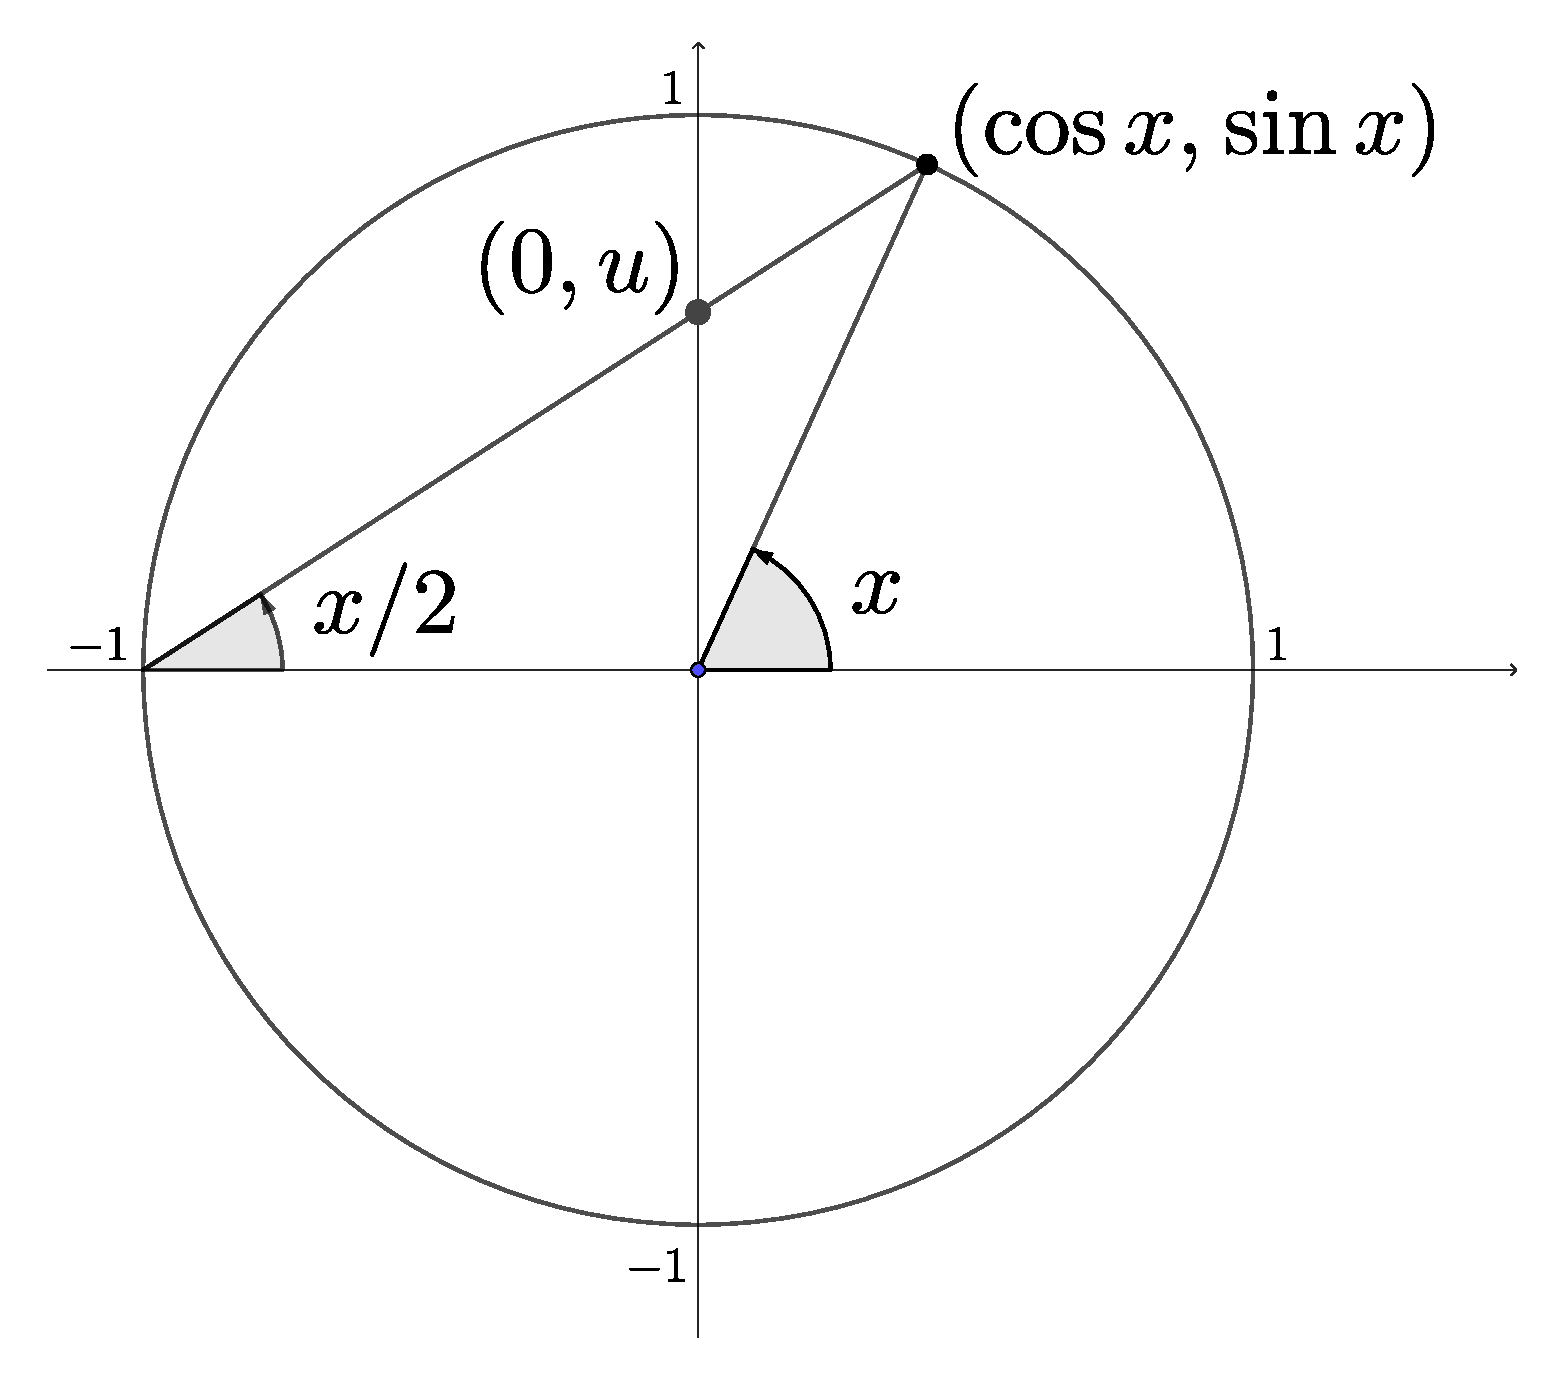
\includegraphics[height=7cm]{03/u-tanx2.pdf}
\end{figure}

\newpage

前ページで紹介した「$\cos x$ と $\sin x$ と定数の四則演算だけで構成される関数」の中でもさらに
\begin{center}
  $\cos^2 x$ と $\sin^2 x$ と $\left( \sin x \right) \left(\cos x\right)$ と定数の四則演算だけで構成される関数
\end{center}
に関しては,変数変換 $\ds u=\tan x$ による置換積分で計算することもできる.例として
\[
  \int_{0}^{\pi/4} \frac{1+\cos^2x}{\sin^2 x + 3 \cos^2 x} \ dx
\]
を計算してみよう.さっそく $\ds u=\tan x$ とおく.このとき,
\[
  \cos^2 x = \frac{1}{1+\tan^2 x} = \frac{1}{1+u^2} \qquad \sin^2 x = 1- \cos^2 x = 1- \frac{1}{1+u^2} = \frac{u^2}{1+u^2}
\]
である.ちなみに,今回は使わないが
\[
  \left( \sin x \right) \left(\cos x\right) = \frac{\sin x}{\cos x}~ \cos^2 x = \left( \tan x \right)\left( \cos^2 x\right)
  = \frac{u}{1+u^2}
\]
である.さらに,
\[
  \frac{du}{dx} = 1+\tan^2 x = 1+u^2 \quad \text{ より } \quad 1 = \frac{1}{1+u^2} \frac{du}{dx} 
\]
である.また,積分範囲は $
\begin{array}{c|ccc}
  x & 0 & \to & \pi/4\\ \hline
  u & 0 & \to & 1
\end{array}
$ と変換されるので,この積分は次のように計算できる.
\[
  \begin{aligned}
    \int_{0}^{\pi/4} \frac{1+\cos^2x}{\sin^2 x + 3 \cos^2 x} \ dx
    &= \int_{0}^{\pi/4} \frac{1+ \frac{1}{1+u^2}}{ \frac{u^2}{1+u^2} + \frac{3}{1+u^2}} \frac{1}{1+u^2}~ \frac{du}{dx} \ dx
      = \int_{0}^{1} \frac{u^2+2}{(u^2+1)(u^2+3)} \ du\\[2ex]
    &= \int_{0}^{1}\left(\frac{\frac{1}{2}}{u^2+1} + \frac{\frac{1}{2}}{u^2+3}\right) \ dx 
      = \frac{1}{2}\left( \Big[ \tan^{-1}u \Big]_{0}^{1} + \left[ \frac{1}{\sqrt{3}}
      \tan^{-1}\frac{u}{\sqrt{3}}\right]_{0}^{1}\right)\\[2ex]
    &=\frac{\pi}{8}  + \frac{\sqrt{3}~\pi}{36}
  \end{aligned}
\]

なお,この変数変換における $u$ と $x$ の関係には下図のような意味づけができる.
\begin{figure}[h]
  \centering
  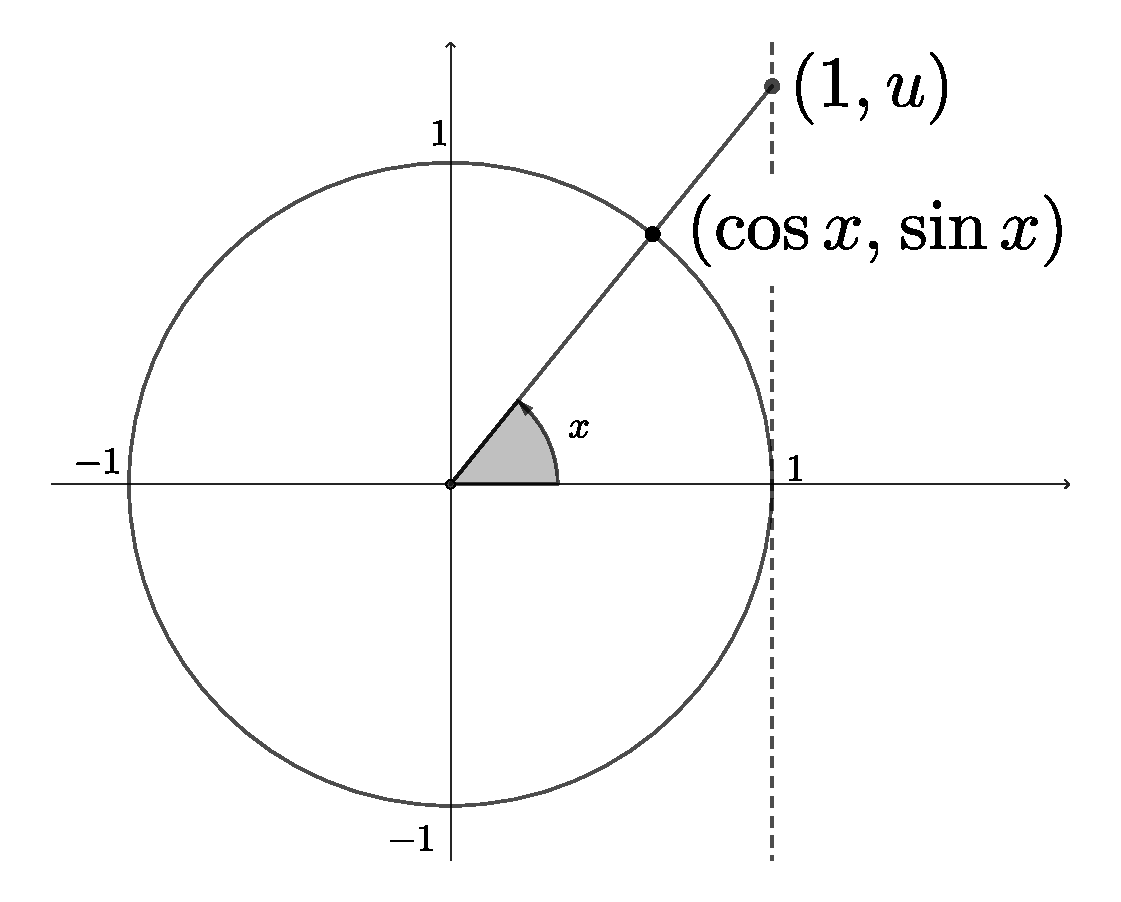
\includegraphics[height=6.5cm]{03/u-tanx.pdf}
\end{figure}

\newpage

さらに特別な場合として,$\left(\sin^m x\right)\left(\cos^nx\right)$ の
積分を考える.例として,以下の $m=2,n=3$ の場合を計算してみるが,$m,n$
の少なくとも一方が奇数なら同様に計算できる.
  \[
    \int_{0}^{\pi/2} \left( \sin^2 x\right) \left( \cos^3 x \right) \ dx
  \]
  これも $\ds u=\tan\frac{x}{2}$ による置換積分で分数関数の積分に帰着できるが,かなり面倒な計算になる.そこで
  \[
    \left( \sin^2 x\right) \left( \cos^3 x\right) = \left( \sin^2 x\right) \left(\cos^2 x\right) \cos x
    = \left( \sin^2 x\right)\left(1-\sin^2 x\right) \cos x
  \]
  と変形してみると,$u=\sin x$ による置換積分がうまくいきそうなことに気
  がつける.実際,$\ds \frac{du}{dx} = \cos x$ であり,積分範囲が
  \[
    \begin{array}{c|ccc}
      x & 0 & \to & \pi/2\\ \hline
      u & 0 & \to & 1
    \end{array}
  \]
  と変換されるので,以下のように割と簡単に計算できてしまう.
  \[
    \int_{0}^{\pi/2} \left( \sin^2 x\right) \left( \cos^3 x\right) \ dx
    = \int_{0}^{1} u^2 \left( 1-u^2\right) \ du = \left[ \frac{u^3}{3} - \frac{u^5}{5}\right]_{0}^{1} = \frac{2}{15}
  \]\\

  続いて,以下の $m=2,n=4$ の場合を計算してみる.$m,n$ の両方が偶数なら同様に計算できる.
  \[
    \int_{0}^{\pi/2} \left( \sin^2 x\right) \left( \cos^4 x\right) \ dx
  \]
  これも $\ds u=\tan\frac{x}{2}$ や $u=\tan x$ による置換積分で分数関数
  の積分に帰着はできるが,まず
  \[
    \left( \sin^2 x\right) \left( \cos^4 x\right) = \left( 1-\cos^2 x\right) \cos^4 x  = \cos^4x - \cos^6 x
  \]
  と変形してみる.ここで半角の公式から
  \[
    \begin{aligned}
      \cos^4 x &= \left( \cos^2 x\right)^2 =
      \left(\frac{1+\cos(2x)}{2}\right)^2 = \frac{1+2\cos(2x) +
        \cos^2(2x)}{4}
      = \frac{1+2\cos(2x) + \frac{1+\cos(4x)}{2}}{4}\\
      &= \frac{3}{8} + \frac{\cos (2x)}{2} + \frac{\cos (4x)}{8}\\ \\
      \cos^6 x &= \left( \cos^2 x\right)^3 = \left(
        \frac{1+\cos(2x)}{2}\right)^3 = \frac{1+3\cos(2x) +
        3\cos^2(2x) + \cos^3(2x)}{8}\\
      &= \frac{1+3\cos(2x) + 3 \frac{1+\cos(4x)}{2}}{8} + \frac{\cos^3(2x)}{8}
      = \frac{5}{16} + \frac{3}{8}\cos(2x) + \frac{3}{16}\cos(4x) + \frac{\cos^3(2x)}{8}
    \end{aligned}
  \]
  なので,この積分は以下のように計算できる.
  \[
    \begin{aligned}
      \int_{0}^{\pi/2} \left(\sin^2 x\right)\left(\cos^4x\right) \ dx
      &= \int_{0}^{\pi/2}\left( \frac{1}{16} + \frac{\cos(2x)}{8} - \frac{\cos(4x)}{16} - \frac{\cos^3(2x)}{8}\right) \ dx\\
      &= \left[\frac{x}{16} + \frac{\sin(2x)}{16} - \frac{\sin(4x)}{64}\right]_{0}^{\pi/2}
      - \frac{1}{8}\int_{0}^{\pi/2}\cos^3(2x) \ dx\\
      & = \frac{\pi}{32} - \frac{1}{8}\int_{0}^{\pi/2}\cos^3(2x) \ dx = \frac{\pi}{32}
    \end{aligned}
  \]
  最後に残った積分は,$\cos^3(2x) = \left(1-\sin^2(2x)\right)
  \cos(2x)$ と変形できるので $u=\sin(2x)$ による置換積分で計算できる.
 


\end{document}
